\documentclass[12pt,AutoFakeBold]{article} 

\usepackage[智能数据挖掘]{XDUreport}  % 科目名称
\problem{对 Twitter 上推文进行情感分析}  % 请在此处填写问题内容
% 其他参数在宏包中进行更改,其中学院,班级,姓名,学号均在sty宏包内进行更改
% \usepackage{fourier}  % 这是 fourier 字体,更柔和 

%% 如果你需要中文的一级标题编号,如“一、”、“二、”等,请把下面两行取消注释
% \RequirePackage{zhnumber} % change section number to chinese
% \titleformat{\section}{\Large\bfseries\rmfamily}{\zhnum{section}、}{0em}{}

% 文档开始
        
\begin{document}

\maketitle
\setcounter{tocdepth}{2}

\tableofcontents  % 生成目录

% 正文标题
\makeatletter
\begin{center}
    \LARGE \textbf{\textsf{\@problem}}
\end{center}
\makeatother

% 正文开始

\section{绪论}

本章节是关于新冠肺炎变种 Omicron 在 2021 年 12 月份时 Twitter 推文的情感分析 (需要科学上网),目的在于利用数据挖掘了解 Twitter 用户的感觉。用 \lstinline[language=Python]|df.info()| 查看数据集各列的数据类型,空值和内存占用情况如下:


\begin{lstlisting}[language=Python]
<class 'pandas.core.frame.DataFrame'>
Int64Index: 48168 entries, 167 to 45168
Data columns (total 16 columns):
 #   Column            Non-Null Count  Dtype         
---  ------            --------------  -----         
 0   id                48168 non-null  int64         
 1   user_name         48168 non-null  object        
 2   user_location     37356 non-null  object        
 3   user_description  45357 non-null  object        
 4   user_created      48168 non-null  datetime64[ns]
 5   user_followers    48168 non-null  int64         
 6   user_friends      48168 non-null  int64         
 7   user_favourites   48168 non-null  int64         
 8   user_verified     48168 non-null  bool          
 9   date              48168 non-null  datetime64[ns]
 10  text              48168 non-null  object        
 11  hashtags          35291 non-null  object        
 12  source            48168 non-null  object        
 13  retweets          48168 non-null  int64         
 14  favorites         48168 non-null  int64         
 15  is_retweet        48168 non-null  bool          
dtypes: bool(2), datetime64[ns](2), int64(6), object(6)
memory usage: 5.6+ MB
\end{lstlisting}

\section{推文分析}

omicron.csv 数据集中有 15168 条推文,在 user\_description, user\_location 和 hashtags 条目有一些空值,分别表示一些用户没有简介、一些用户没有位置信息以及一些推文没有哈希标签。用 \lstinline[language=Python]|df[df.duplicated()]| 可以发现没有重复推文。

\subsection{不同日期推文分析}

在数据中有两列 ('date', 'user\_created') 表示时间,将其转化为 pandas datatime 以便于分析。统计得到不同日期的推文数量柱状图如图 \ref{fig:datecounts} 所示。

\begin{figure}[htbp]
	\centering
    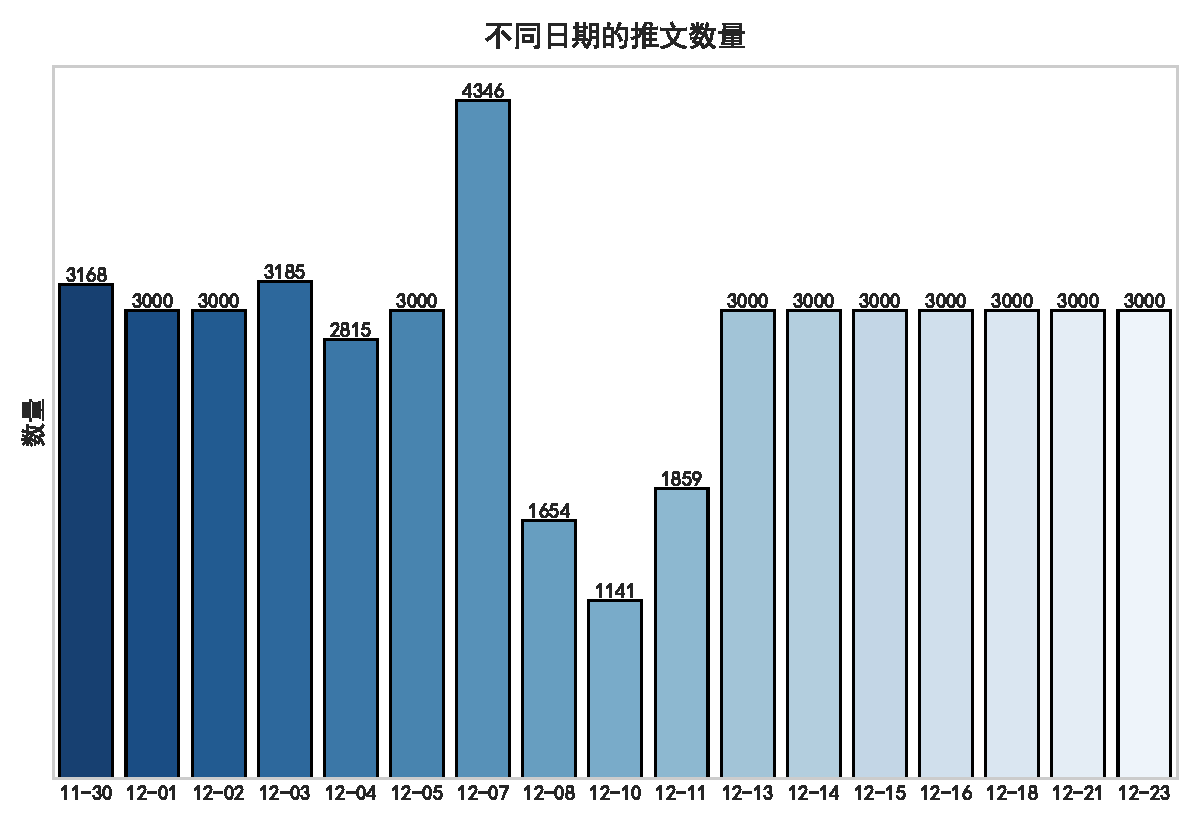
\includegraphics[width=0.7\textwidth]{datecounts.pdf}
    \caption{不同日期的推文数量柱状图} \label{fig:datecounts}
\end{figure}

可以看出关于 Omicron 推文数量最高的在 12 月 7 日,值得注意的是,12 月 13 日和 12 月 23 日之间的推文数量是恒定的,都是 3000 条,这可能是由于每天的推文爬取限制。

\subsection{24 小时内不同时间的推文分析}

同理可以统计得到 24 小时内不同时间的推文数量柱状图如图 \ref{fig:hourcounts} 所示。

\begin{figure}[htbp]
	\centering
    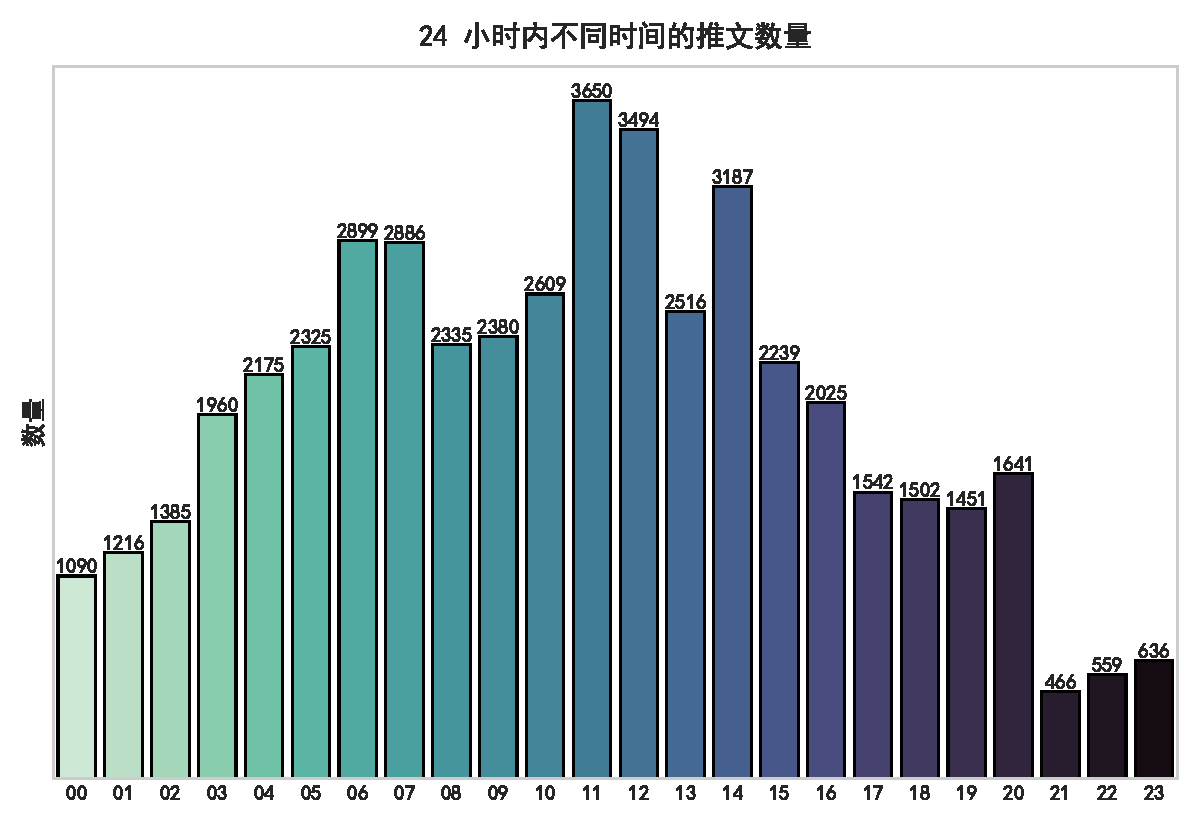
\includegraphics[width=0.7\textwidth]{hourcounts.pdf}
    \caption{24 小时内不同时间的推文数量柱状图} \label{fig:hourcounts}
\end{figure}

可以看到从 00:00 到 6:00 的有上升趋势,从 6:00 到 9:00 有下降趋势,以及从 9:00 到 12:00 的僵硬上升。

\subsection{不同国家推文分析}

通过代码 \lstinline[language=Python]|df['user\_location'].value\_counts()| 可以发现用户位置不总是国家,我们可以通过 pycountry 这个库提取出国家。创建新列表属性 “国家”,找不到国家则为空值。接着统计推文数大于 30 的国家推文数,不同国家的推文数量柱状图如图 \ref{fig:countrycounts} 所示。

\begin{figure}[htbp]
	\centering
    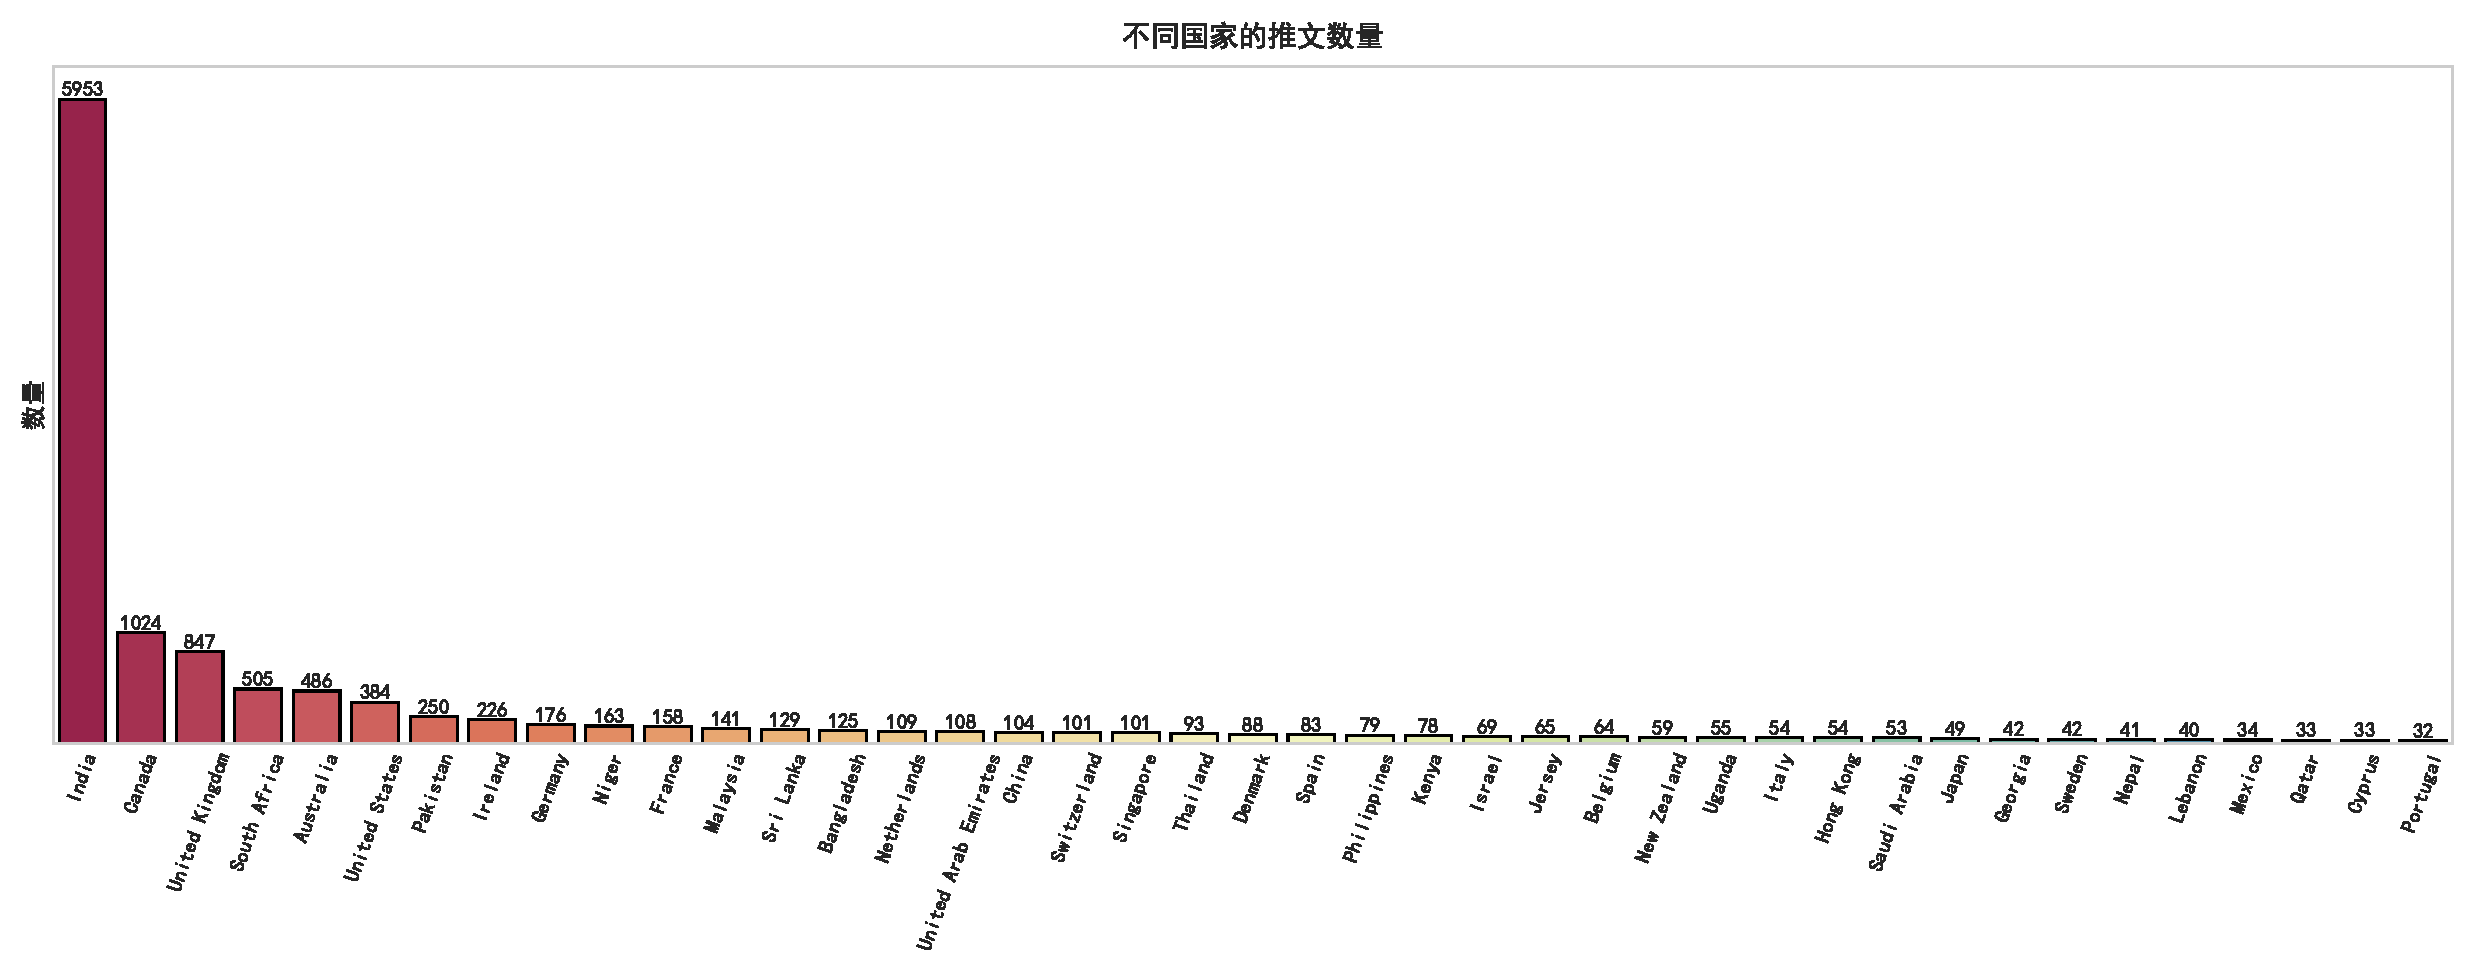
\includegraphics[width=\textwidth]{countrycounts.pdf}
    \caption{不同国家的推文数量柱状图} \label{fig:countrycounts}
\end{figure}

\subsection{推文点赞分析}

通过 \lstinline[language=Python]|fav\_tweets = df[['text','favorites']].sort\_values('favorites', ascending=False)| 可以将推文按点赞数降序排序,然后通过 \lstinline[language=Python]|fav\_tweets['text'].iloc[:10].values| 找出点赞数前 10 的推文内容如图 \ref{fig:fav1} 所示。

\begin{figure}[htbp]
	\centering
    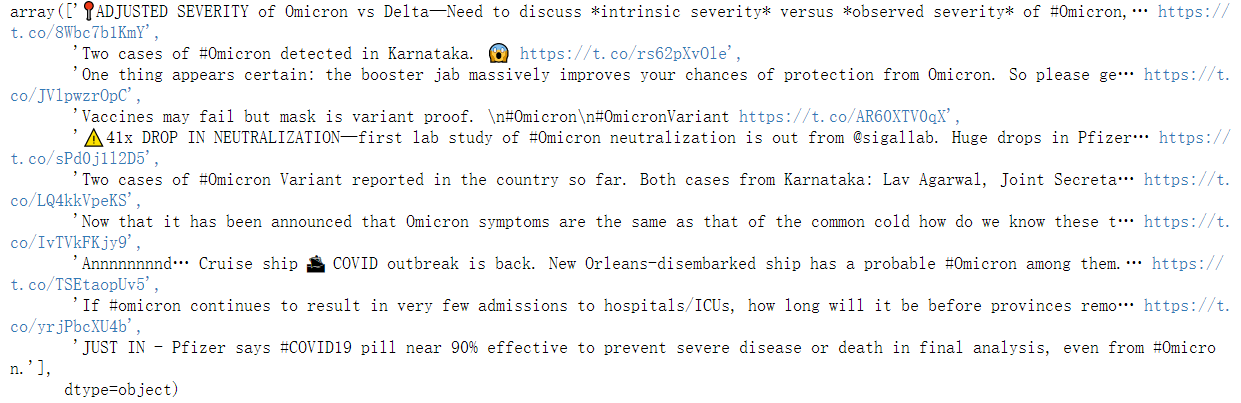
\includegraphics[width=0.7\textwidth]{fav1.png}
    \caption{点赞数前 10 的推文} \label{fig:fav1}
\end{figure}

\subsection{推文转推分析}

通过 \lstinline[language=Python]|retweets = df[['text','retweets']].sort\_values('retweets', ascending=False)| 可以将推文按转推数降序排序,然后通过 \lstinline[language=Python]|retweets['text'].iloc[:10].values| 找出转推数前 10 的推文内容如图 \ref{fig:fav2} 所示。

\begin{figure}[htbp]
	\centering
    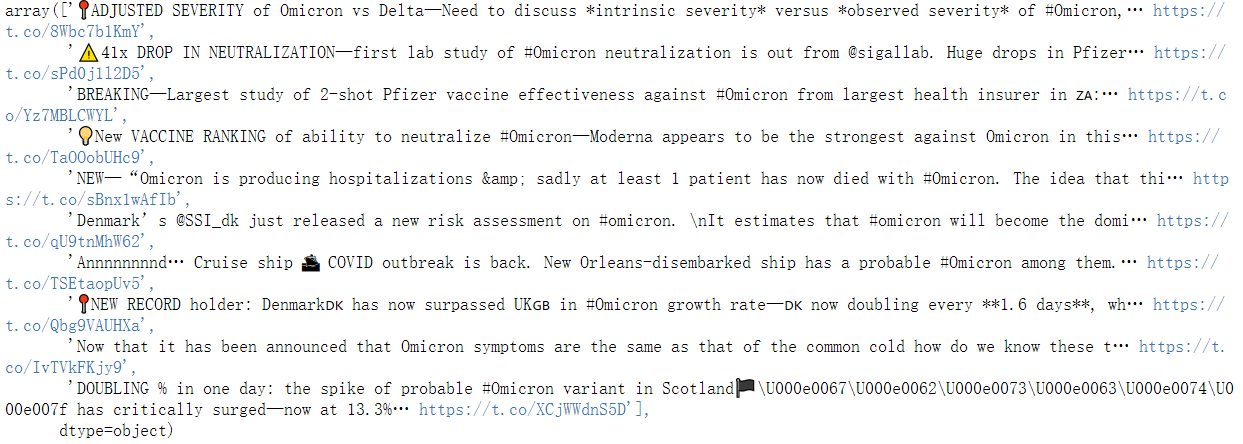
\includegraphics[width=0.7\textwidth]{fav2.png}
    \caption{转推数前 10 的推文} \label{fig:fav2}
\end{figure}

可以发现点赞数和转推数最多的推文都是由美籍华裔健康经济学家 Eric Feigl-Ding 发布的关于 Omicron 病毒的评价,这与他庞大的粉丝数量是密切相关的。

\section{推文情感分析}

首先对推文数据用自定义函数进行数据清洗,主要是去掉表情和一些特殊字符并改成小写。清洗后文本长度如图 \ref{fig:cleanedtext} 所示·,观察到一些推文单词数很少,少于 10 个单词的文本柱状图如图 \ref{fig:less10} 所示。在后续分析中将去掉少于 5 个单词的推文。

\begin{figure}[htbp]
	\centering
	\begin{minipage}[t]{0.48\textwidth}
		\centering
		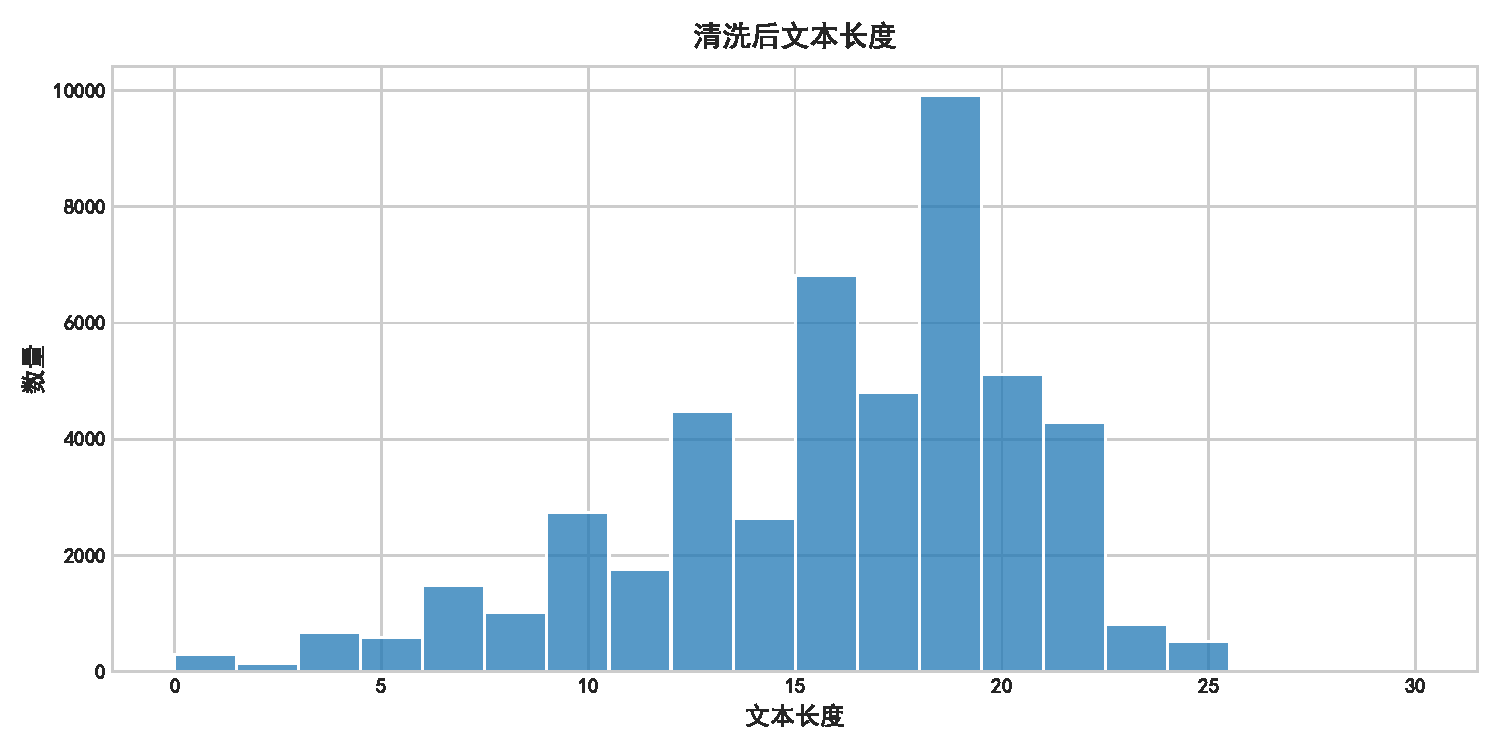
\includegraphics[width=\textwidth]{cleanedtext.pdf}
		\caption{清洗后文本长度} \label{fig:cleanedtext}
	\end{minipage}
	\begin{minipage}[t]{0.48\textwidth}
		\centering
		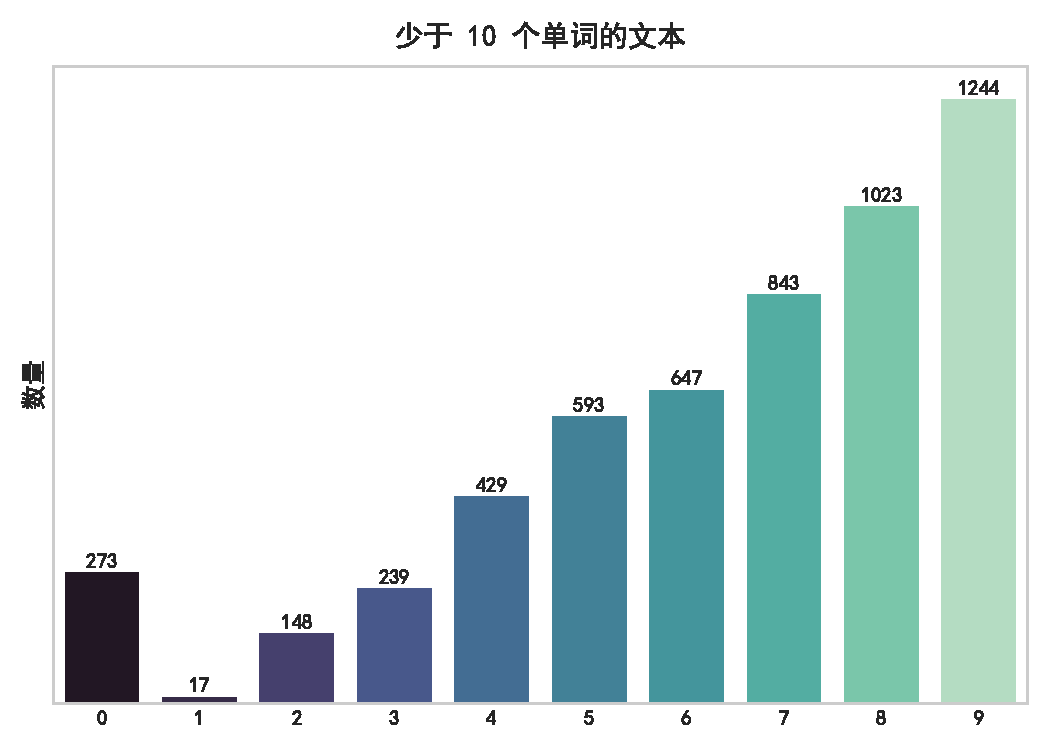
\includegraphics[width=\textwidth]{less10.pdf}
		\caption{少于 10 个单词的文本柱状图} \label{fig:less10}
	\end{minipage}
\end{figure}

接下来用 NLTK 和 TextBlob 分别进行情感分析,我将绘制每种方法的词云,首先需要添加一些 stopwords,指所有类别推文都共享的词,比如 'covid' 和 'omicron' 等等。

\subsection{正面推文}

正面推文词云如图 \ref{fig:wordcloud1} 所示。综合两种方法得到的综合正面推文词云如图 \ref{fig:wordcloud2} 所示。综合正面推文如下:

\begin{lstlisting}[language=Python]
array(['wonderful project sir this project looks very interesting i am interested and i will support this',
       'outstanding thread from one of the best cc omicron covid19',
       'good join the club happily membership is growing omicron',
       'good evening dear friend be careful with omicron',
       'nice looks like you are better protected against omicron then me',
       'omicron alert level4 help raise awareness bettermasks good fit amp filtration is key ffp2 cloth mask good fit over',
       'happy holidays mani xmas omicron',
       'this is nuts do better health care do better testingtestingtesting covid19 omicron',
       'discover and share your best business content download the best app gt theeconomist',
       'wise words from a wise man omicron'], dtype=object)
\end{lstlisting}

\begin{figure}[htbp]
	\centering
    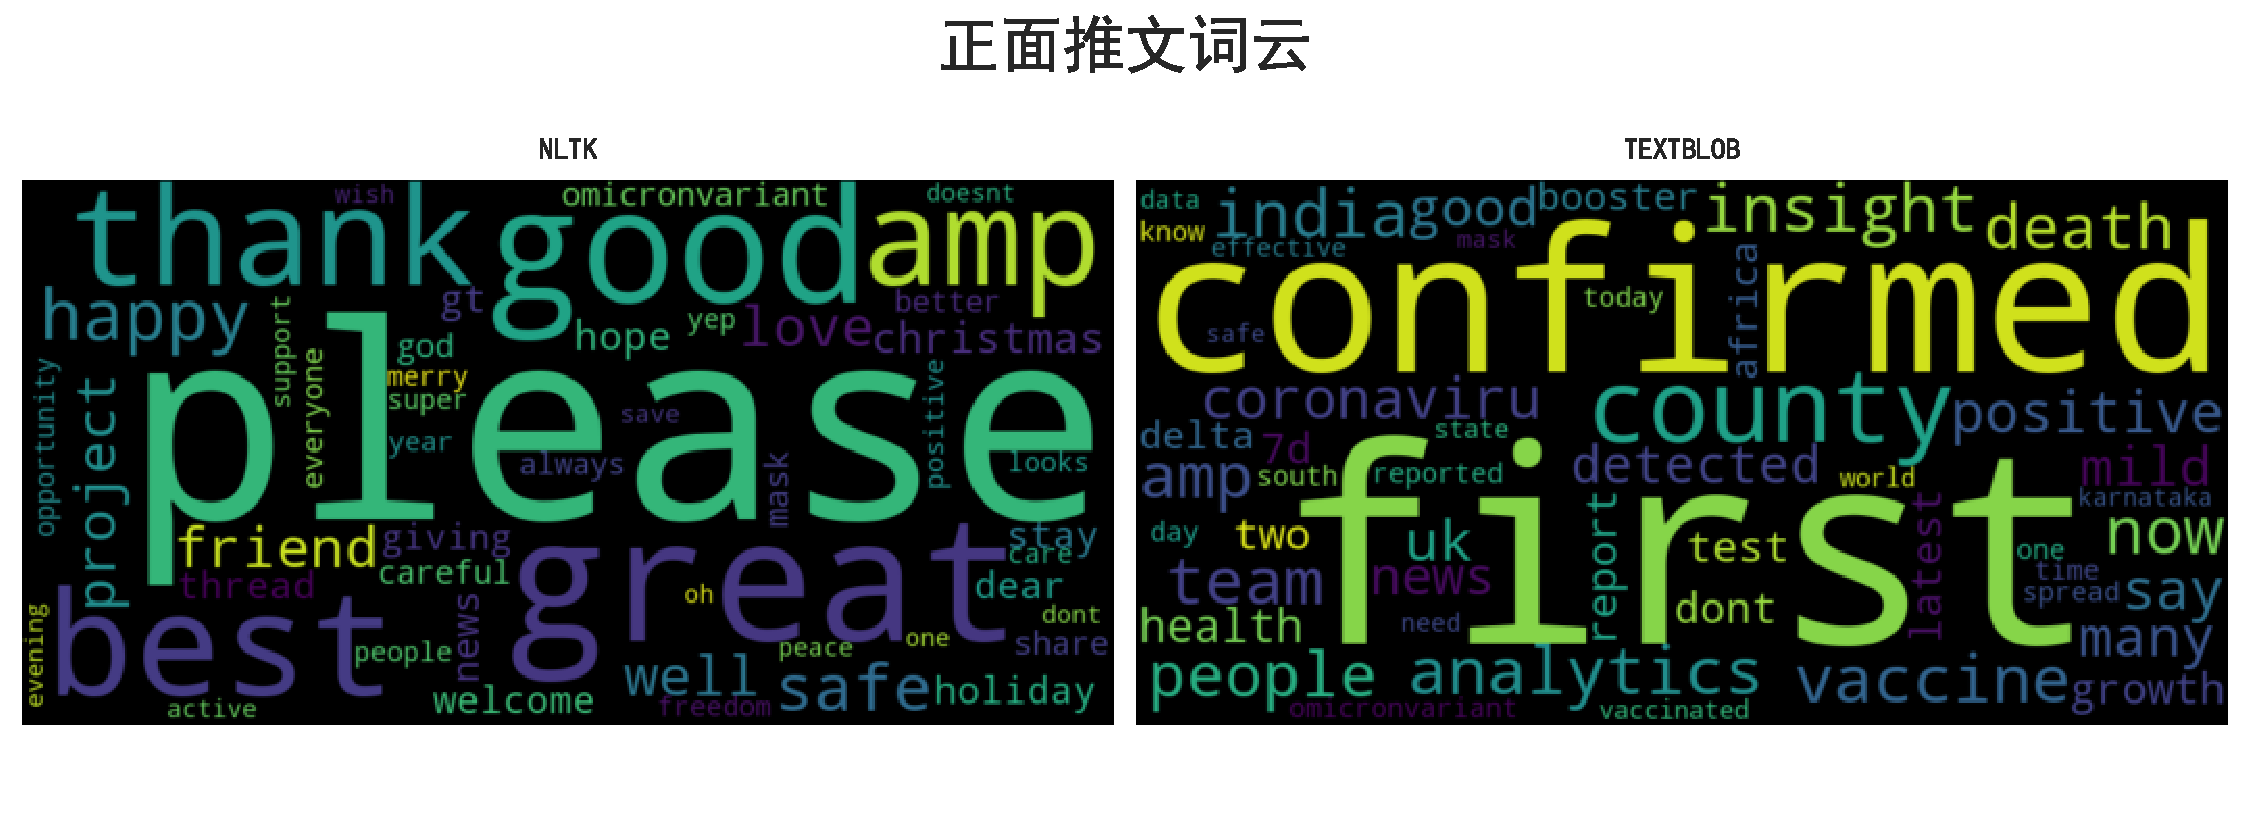
\includegraphics[width=0.7\textwidth]{wordcloud1.pdf}
    \caption{正面推文词云} \label{fig:wordcloud1}
\end{figure}

\begin{figure}[htbp]
	\centering
    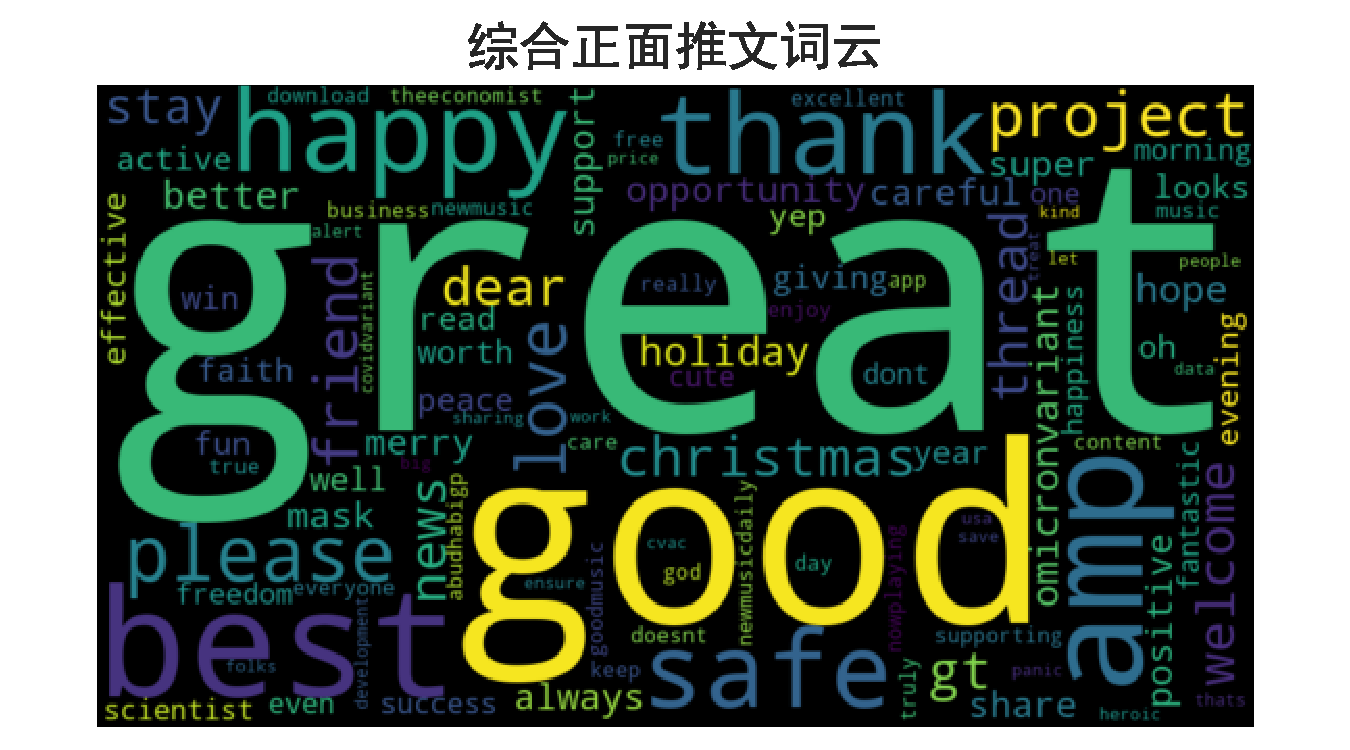
\includegraphics[width=0.6\textwidth]{wordcloud2.pdf}
    \caption{综合正面推文词云} \label{fig:wordcloud2}
\end{figure}

\subsection{负面推文}

负面推文词云如图 \ref{fig:wordcloud3} 所示。综合两种方法得到的综合负面推文词云如图 \ref{fig:wordcloud4} 所示,可以看出这些词确实都非常负面。综合负面推文如下:

\begin{lstlisting}[language=Python]
array(['omicron is less severe buy risk',
       'omicron you crazy son of a bitch',
       'hospitalizations lowest death rate lowest severity lowest ippudanna aa fear mongering aapesi lock down l',
       'flu omicron serious chance of serious illness',
       'omicron sorry omicon covid scam',
       'they mad because no one is scared of omicron',
       'omicron bad could be worse get boosted good night',
       'open door fucker via f1finale idiot omicron',
       'america ohio americasgottalent dead another death jayjayphillips was discovered dead',
       'shocking racism omicron africa europe'], dtype=object)
\end{lstlisting}

\begin{figure}[htbp]
	\centering
    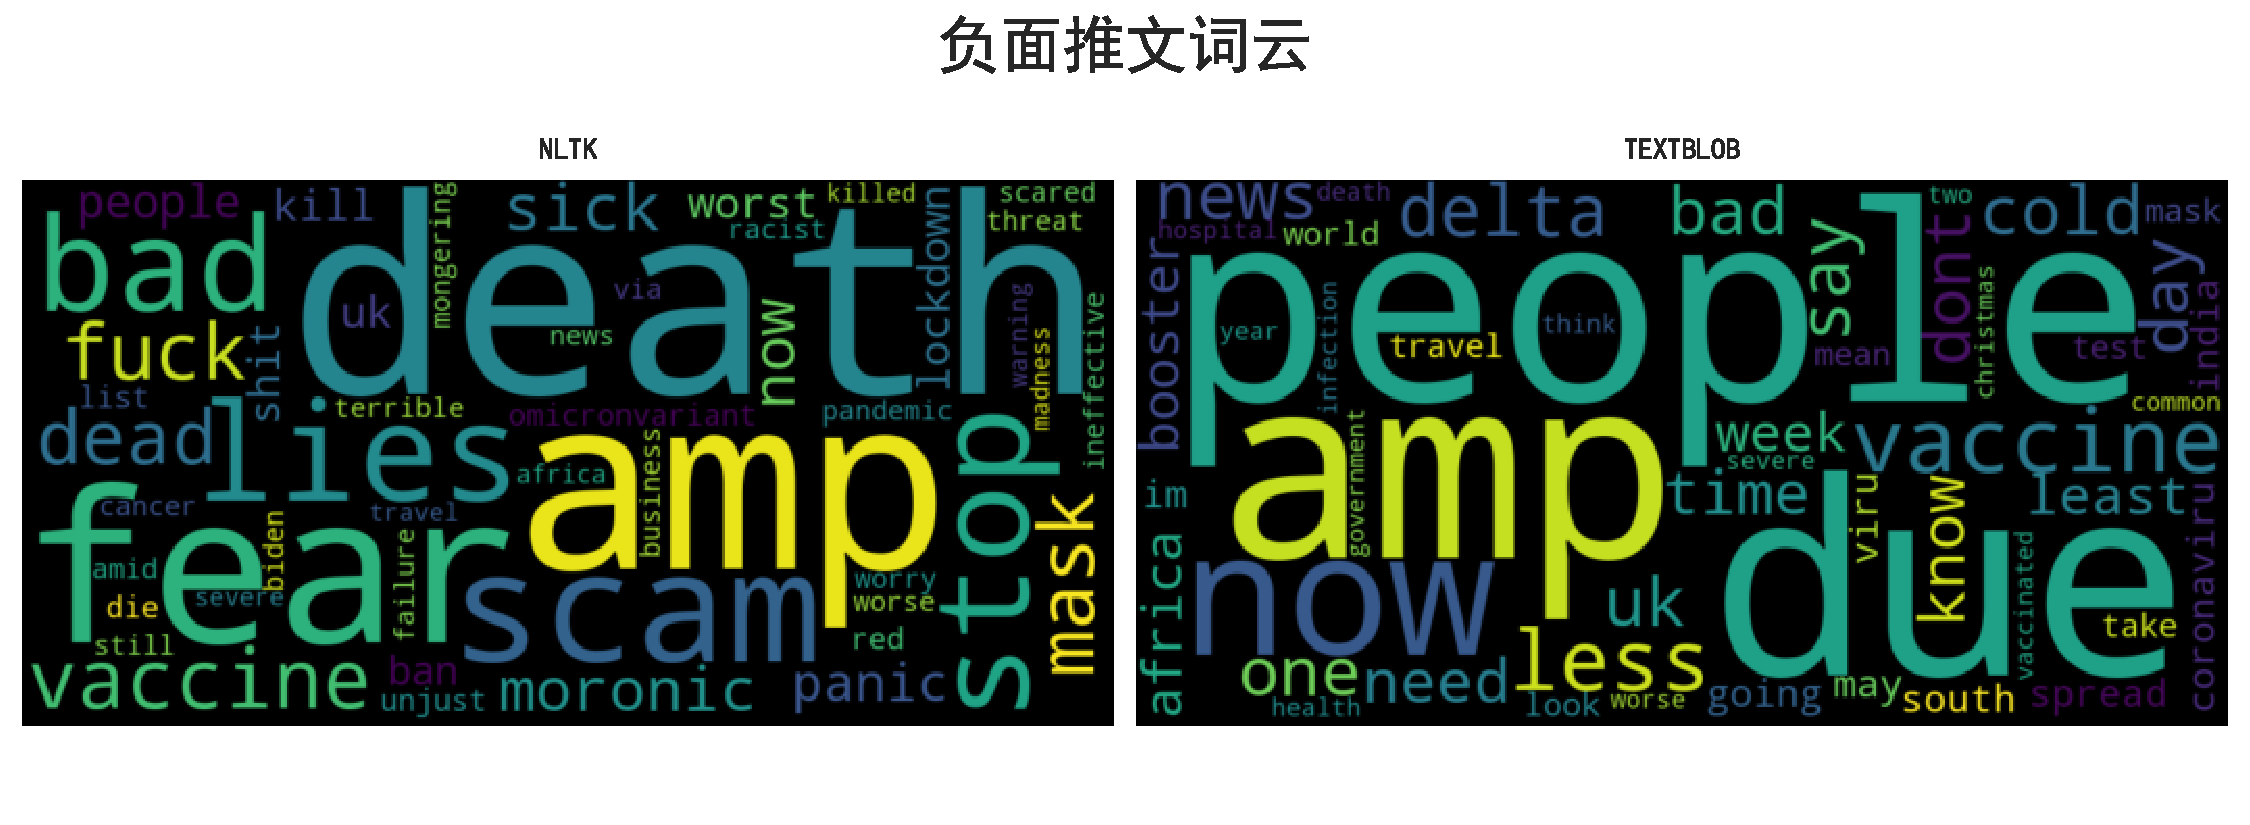
\includegraphics[width=0.7\textwidth]{wordcloud3.pdf}
    \caption{负面推文词云} \label{fig:wordcloud3}
\end{figure}

\begin{figure}[htbp]
	\centering
    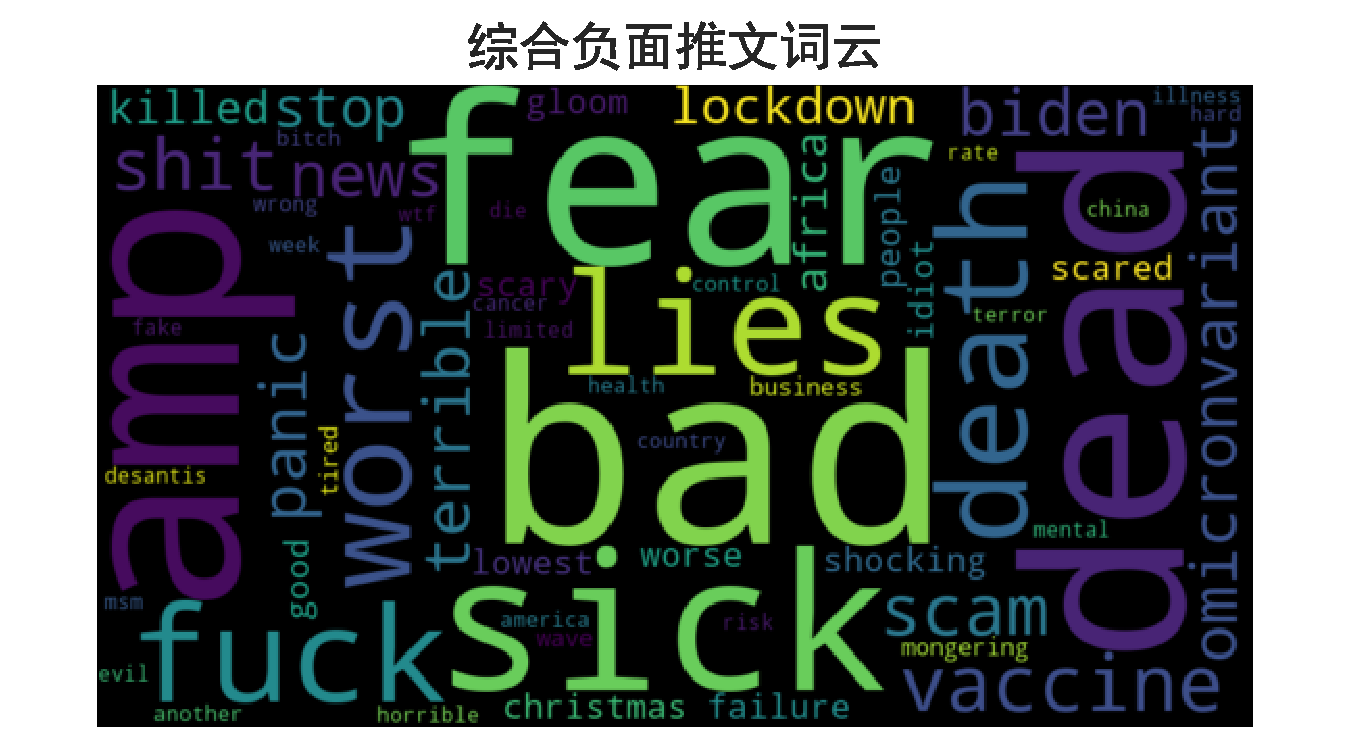
\includegraphics[width=0.6\textwidth]{wordcloud4.pdf}
    \caption{综合负面推文词云} \label{fig:wordcloud4}
\end{figure}

% % 参考文献,此处以 MLA 引用格式为例

% \begin{thebibliography}{9}
%     \bibitem{1} Clemente, Filipe Manuel, et al. "General network analysis of national soccer teams in FIFA World Cup 2014." \emph{International Journal of Performance Analysis in Sport} 15.1 (2015): 80-96.
%     \bibitem{3} Dijkstra, Edsger Wybe. "A Note on Two Problems in Connexion With Graphs." \emph{Numerische Mathematik} 1(1959):269-271.
%     \bibitem{4} Ahnert, Sebastian E., et al. "Ensemble approach to the analysis of weighted networks.." \emph{Physical Review E} 76.1 (2007).
%     \bibitem{5} Wong, J. A. Hartiganm. A. . "Algorithm AS 136: A K-Means Clustering Algorithm." \emph{Journal of the Royal Statistical Society. Series C (Applied Statistics)} 28.1(1979):100-108.
%     \bibitem{6} Buldu, J. M., et al. "Defining a historic football team: Using Network Science to analyze Guardiola’s F.C. Barcelona." \emph{Scientific Reports} 9.1 (2019): 1-14.
%     \bibitem{7} \emph{Balotelli sends Italy past Germany}. (2012). Retrieved December 10, 2014, from\url{https://www.uefa.com/uefaeuro/season=2012/matches/round=15174/match=2003379/index.html}
%     \bibitem{8} Sigari, Mohamad Hoseyn, et al. "Counterattack detection in broadcast soccer videos using camera motion estimation." \emph{international symposium on artificial intelligence} (2015): 101-106.
%     \bibitem{9} Abdelmahmoud Hassan Elsheikh. \emph{Effect of Leadership Intensity on Integrating Some Formal and Informal Organizational Efforts for Community Development in Khartoum Province}. 2016.
% \end{thebibliography}


% \includepdf[pages={1,2}]{Memo.pdf} 
% 可以直接导入pdf页面
% \newpage
% \begin{appendices}  % 附录环境
% \section{附录}
% \end{appendices}

\end{document}  % 结束